\item Para este objetivo tuvimos que filtrar de nuevo como se ve en la figura \ref{filtrosnuevos}, ya que solo nos pedían los estados de Veracruz y Tamaulipas y además teniamos que dividir el año 2020; después de esto pasamos a crear un guardado e incorporarlo en el documento, para hacer una predicción como se muestra en la figura \ref{tercerfiltro}, de igual manera cargamos los datos reales y los graficamos enseguida se adjuntan ambas imágenes.
\begin{figure}[h]
    \centering
    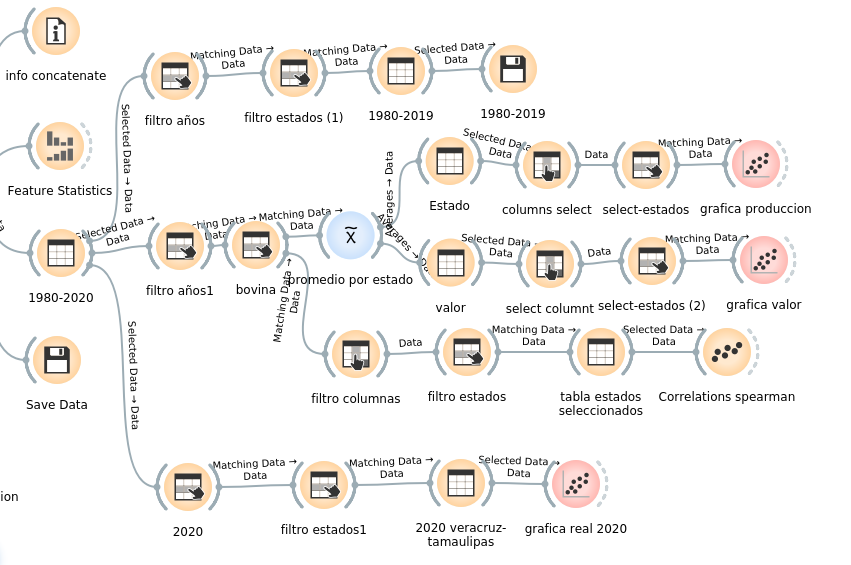
\includegraphics[scale = 0.4]{imagenes/Orange2.png}
    \caption{Filtros Nuevos}
    \label{filtrosnuevos}
\end{figure}
\begin{figure}[h]
    \centering
    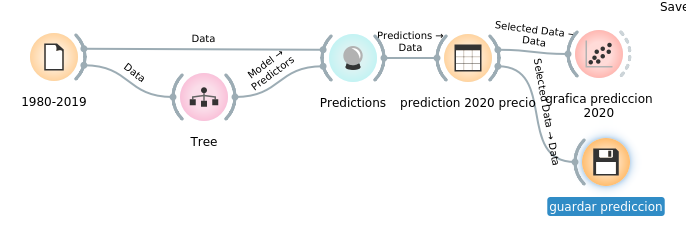
\includegraphics[scale = 0.5]{imagenes/orange3.png}
    \caption{Tercer filtro}
    \label{tercerfiltro}
\end{figure}
\begin{figure}[htb!]
\begin{minipage}[b]{0.5\linewidth} %Una minipágina que cubre la mitad de la página
\centering
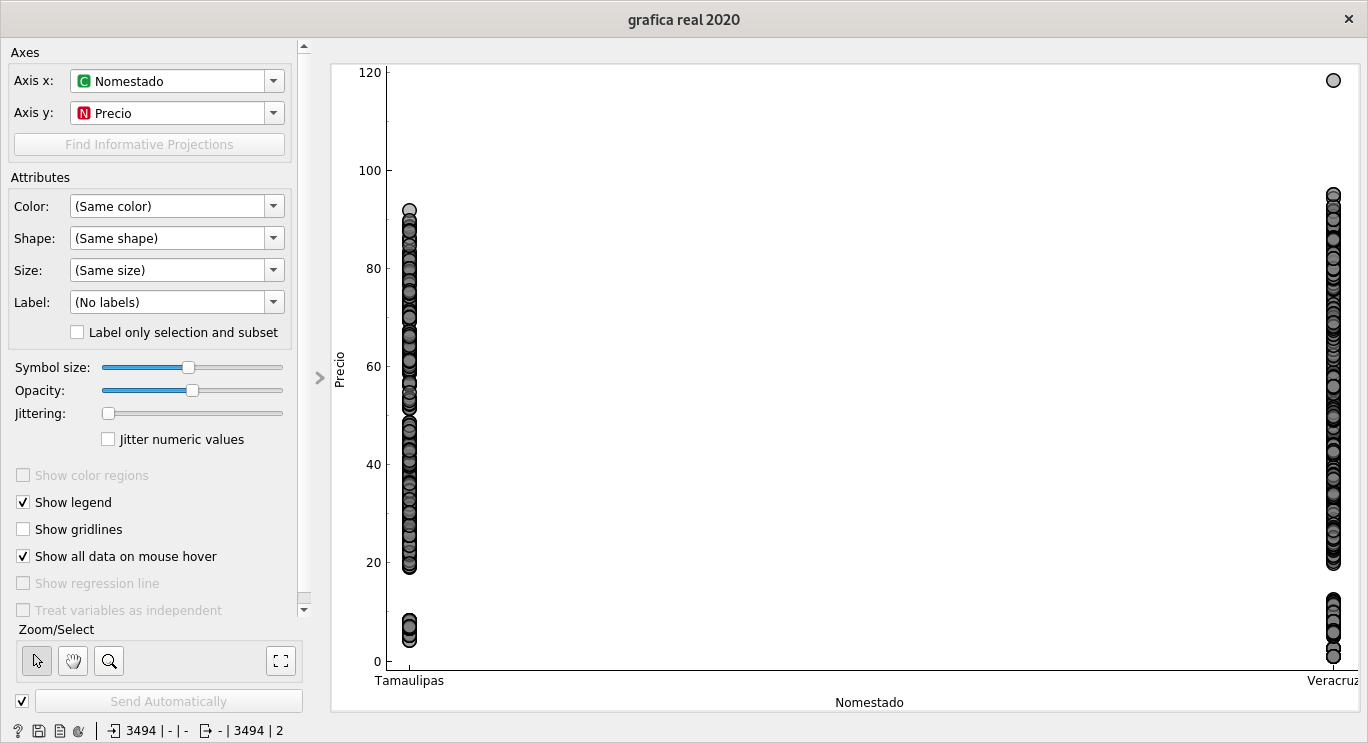
\includegraphics[width=8cm]{imagenes/grafica-real-2020.png}
    \caption{Gráfica real 2020}
    \label{graficareal}
\end{minipage}
\hspace{0.5cm} % Si queremos tener un poco de espacio entre las dos figuras
\begin{minipage}[b]{0.5\linewidth}
\centering
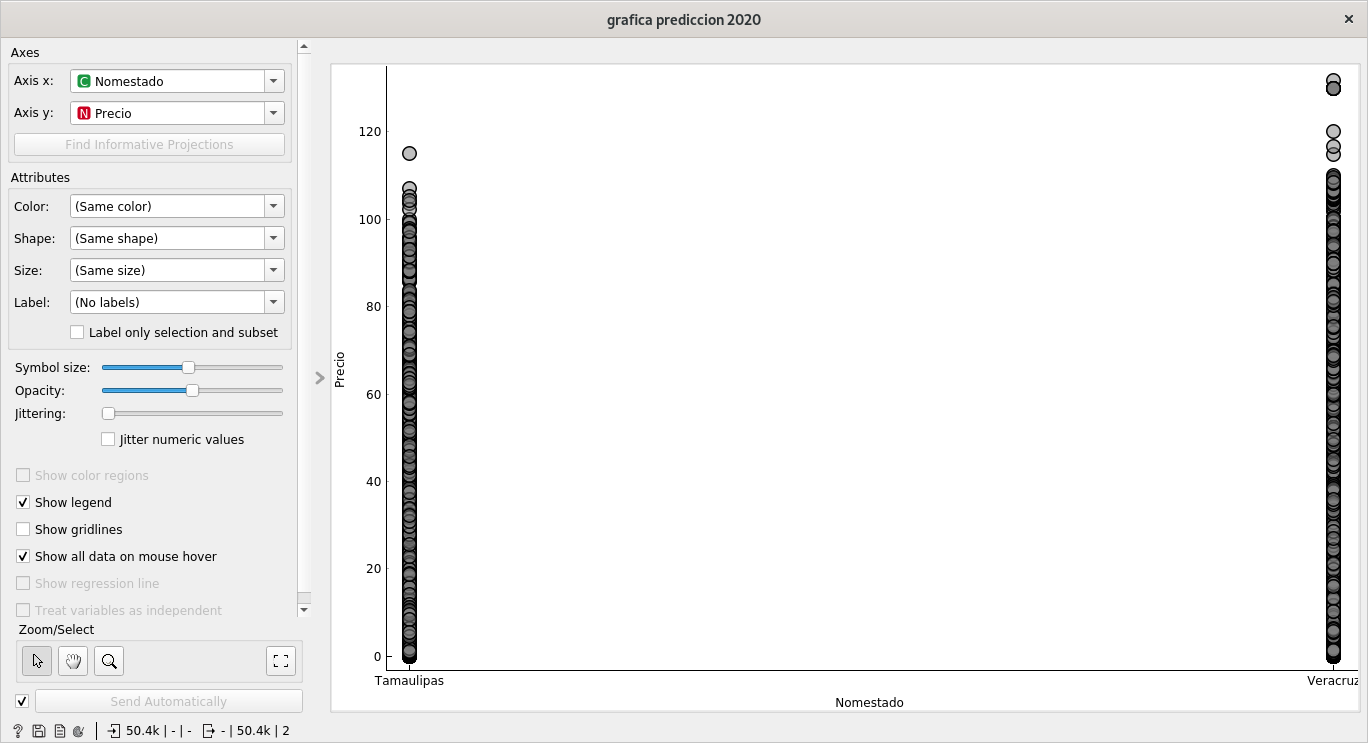
\includegraphics[width=8cm]{imagenes/grafica-prediccion.png}
    \caption{Gráfica predicción 2020}
    \label{graficaprediccion}
\end{minipage}
\end{figure}
\newpage
Como podemos ver la gráfica entre ambas es demasiado similar.
Entonces de cierto modo podemos decir que nuestra predicción es demasiado cerca a los datos reales.